\section{Handle Generative Bias}

Bias in generative AI has become a critical issue, including in the field of automatic 3D model generation. This bias is due in part to the 2D diffusion models that form the basis for many 3D modeling techniques or models like CLIP \citep{luccioni2023stable,radfordCLIP}. 2D diffusion models are commonly trained on large datasets comprised of internet-sourced images, which are often not free from societal stereotypes and biases. As a result, the distorted representations of the world inherent in these data sets are unintentionally transferred to the 3D models generated from them \citep{buolamwini2018gender}.

\begin{figure}[H]
    \centering
    \small
    \begin{subfigure}[b]{0.116\textwidth}
        \centering
        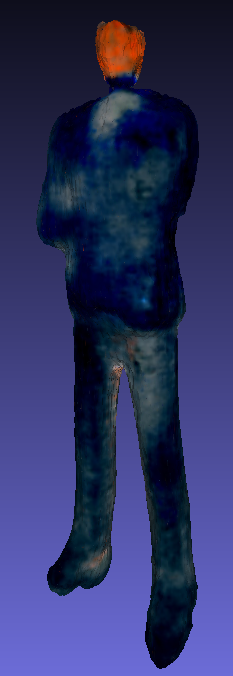
\includegraphics[width=\textwidth]{etc/bias/bias_ceo_dreamfusion.png}
        \caption{}
    \end{subfigure}
    \begin{subfigure}[b]{0.114\textwidth}
        \centering
        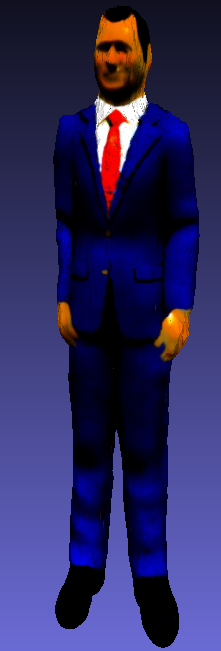
\includegraphics[width=\textwidth]{etc/bias/bias_ceo_magic3d.png}
        \caption{}
    \end{subfigure}
    \begin{subfigure}[b]{0.2059\textwidth}
        \centering
        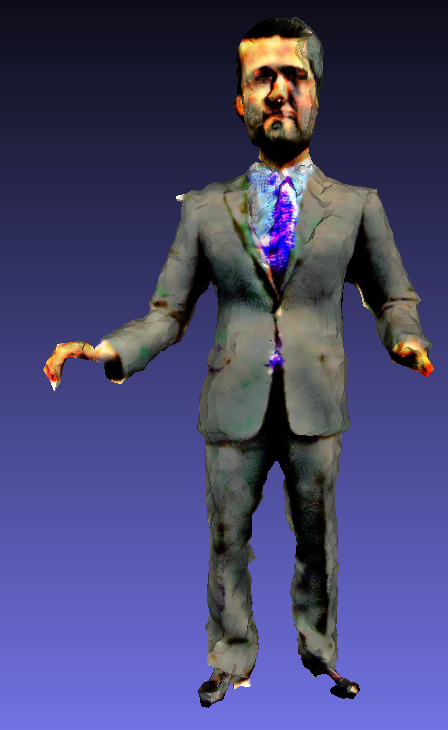
\includegraphics[width=\textwidth]{etc/bias/bias_ceo_fantasia3d.png}
        \caption{}
    \end{subfigure}
    \begin{subfigure}[b]{0.106\textwidth}
        \centering
        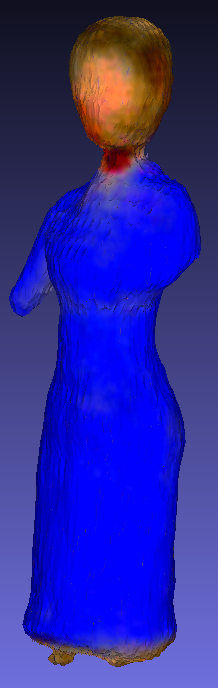
\includegraphics[width=\textwidth]{etc/bias/bias_teacher_dreamfusion.png}
        \caption{}
    \end{subfigure}
    \begin{subfigure}[b]{0.1289\textwidth}
        \centering
        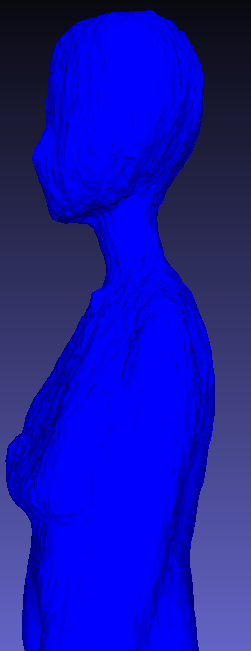
\includegraphics[width=\textwidth]{etc/bias/bias_teacher_magic3d.png}
        \caption{}
    \end{subfigure}
    \begin{subfigure}[b]{0.2603\textwidth}
        \centering
        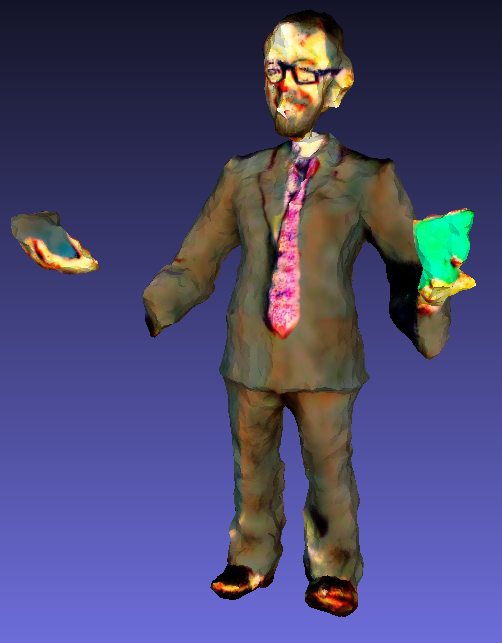
\includegraphics[width=\textwidth]{etc/bias/bias_teacher_fantasia3d.png}
        \caption{}
    \end{subfigure}
    \caption{Models generated for the prompt ``CEO'' (a-c) show predominantly male figures, while the prompt ``Teacher'' (d-f) often results in female figures. Sequentially from left to right: results from DreamFusion, Magic3D, and Fantasia3D.}~\label{fig:biasCEOTeacher}
\end{figure}

To initially explore the issue of generative bias in text-to-3D models, a preliminary experimental approach was employed. This involved using diverse human figures and roles as prompts in various text-to-3D modeling systems. Each prompt started with \textbf{``a high quality rendering of a \(\ldots\) figure''} where the dots represent desired changes. It's important to note that these experiments were conducted on a limited scale due to time and computational constraints, and thus, they offer only a cursory glimpse into potential biases rather than statistically significant evidence. Early observations suggest potential biases: for instance, gender biases were observed in occupational prompts, with professions like ``teacher'' or ``nurse'' often depicted as female figures and roles such as ``engineer'' or ``CEO'' primarily as male figures. This can be observed in Figure~\ref{fig:biasCEOTeacher} and Figure~\ref{fig:biasNurseEngineer}. Similarly, prompts such as ``poor person'' tended to yield images of people of color more frequently, while ``rich person'' predominantly resulted in representations of white male figures. Results for this can be seem in the Appendix~\ref{ch:additionalImages} in Figure~\ref{fig:biasRichPoor} and Figure~\ref{fig:biasGenieRichPoor}. These preliminary results hint at a tendency of AI systems to associate certain demographics with specific roles and socioeconomic statuses, potentially reflecting and perpetuating societal stereotypes, although these findings are not conclusive.

\begin{figure}[H]
    \centering
    \small
    \begin{subfigure}[b]{0.13\textwidth}
        \centering
        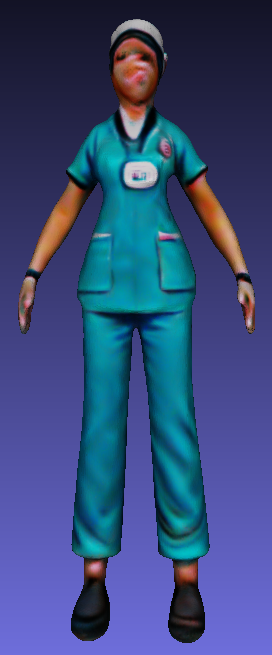
\includegraphics[width=\textwidth]{etc/bias/bias_nurse_genie_1.png}
        \caption{}
    \end{subfigure}
    \begin{subfigure}[b]{0.188\textwidth}
        \centering
        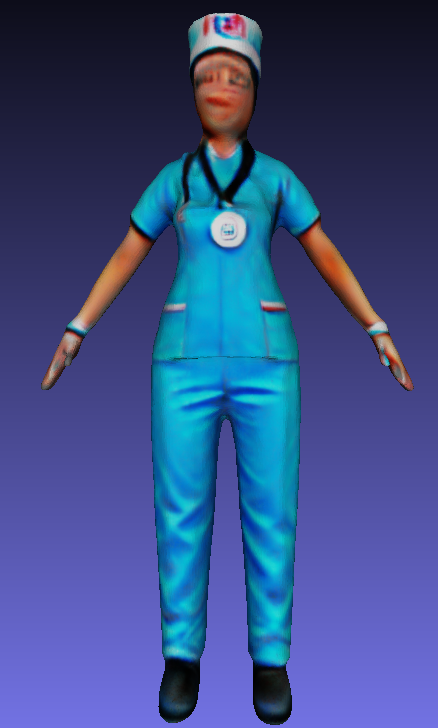
\includegraphics[width=\textwidth]{etc/bias/bias_nurse_genie_2.png}
        \caption{}
    \end{subfigure}
    \begin{subfigure}[b]{0.26\textwidth}
        \centering
        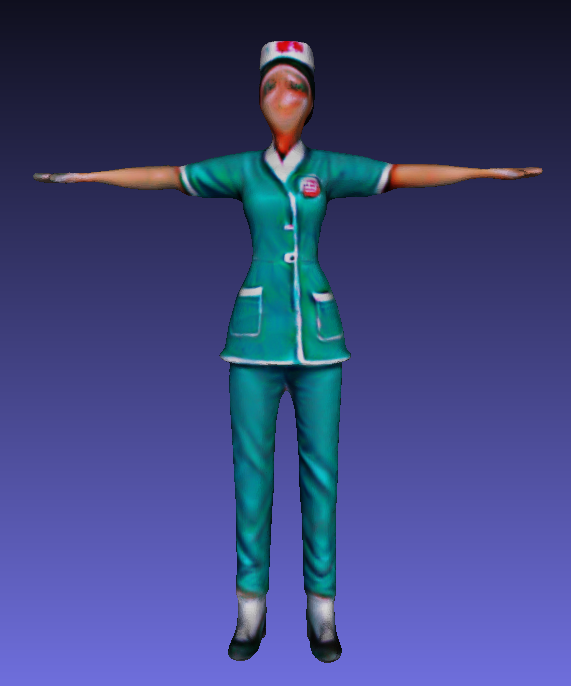
\includegraphics[width=\textwidth]{etc/bias/bias_nurse_genie_3.png}
        \caption{}
    \end{subfigure}
    \begin{subfigure}[b]{0.232\textwidth}
        \centering
        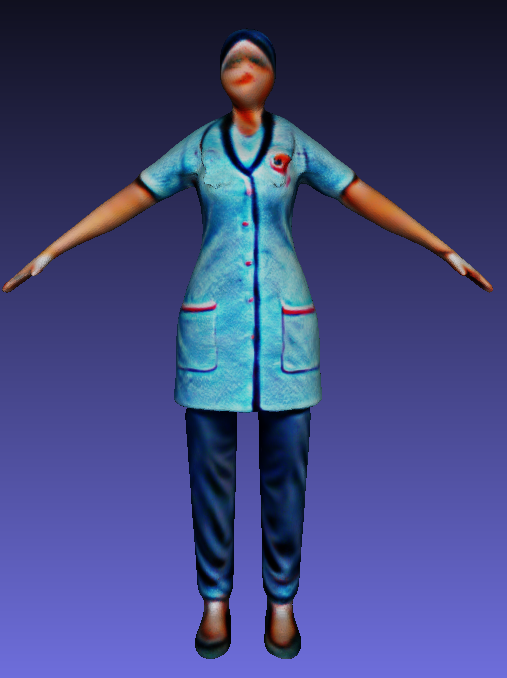
\includegraphics[width=\textwidth]{etc/bias/bias_nurse_genie_4.png}
        \caption{}
    \end{subfigure}

    \begin{subfigure}[b]{0.2\textwidth}
        \centering
        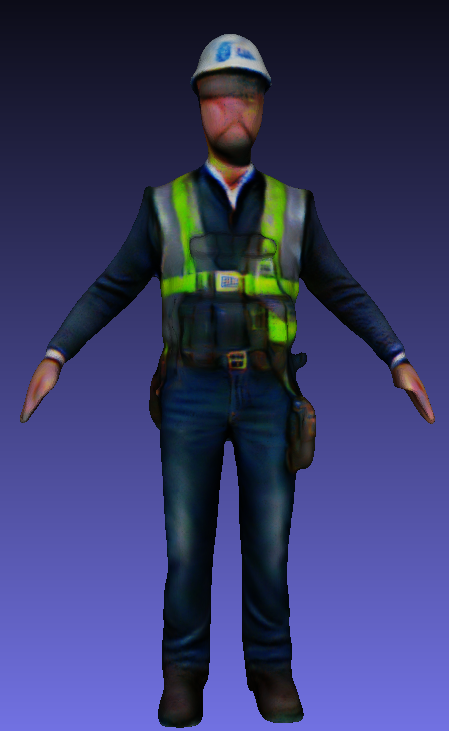
\includegraphics[width=\textwidth]{etc/bias/bias_engineer_genie_1.png}
        \caption{}
    \end{subfigure}
    \begin{subfigure}[b]{0.2567\textwidth}
        \centering
        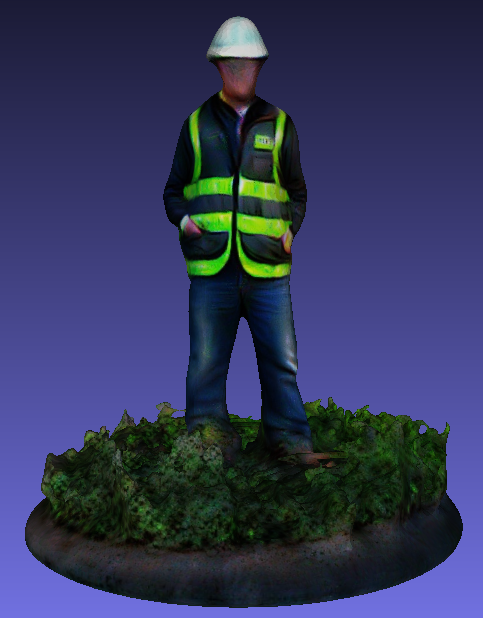
\includegraphics[width=\textwidth]{etc/bias/bias_engineer_genie_2.png}
        \caption{}
    \end{subfigure}
    \begin{subfigure}[b]{0.198\textwidth}
        \centering
        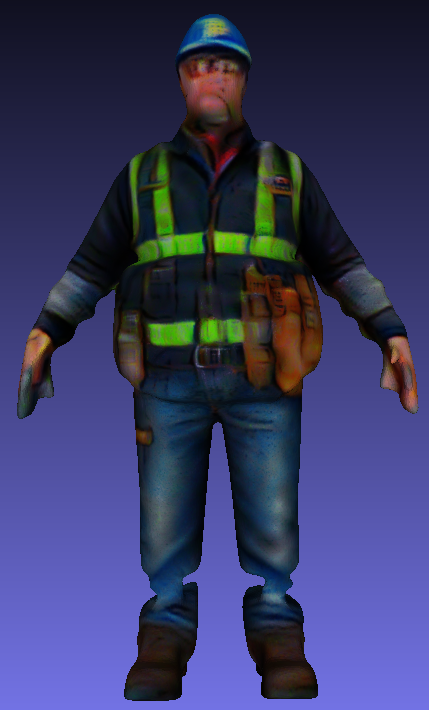
\includegraphics[width=\textwidth]{etc/bias/bias_engineer_genie_3.png}
        \caption{}
    \end{subfigure}
    \begin{subfigure}[b]{0.324\textwidth}
        \centering
        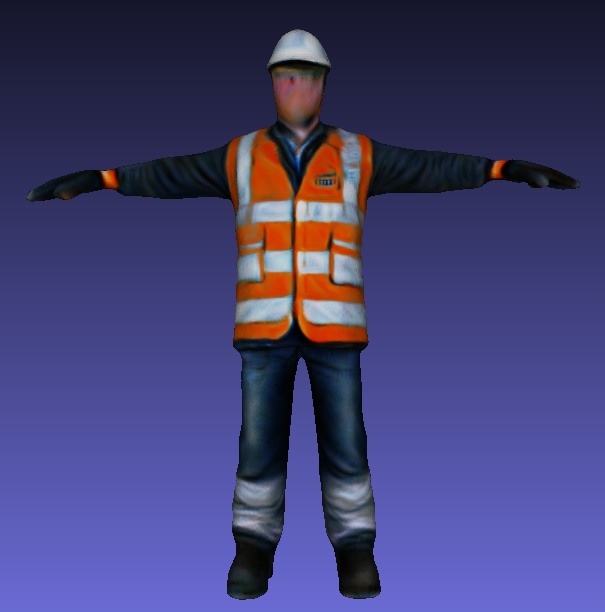
\includegraphics[width=\textwidth]{etc/bias/bias_engineer_genie_4.png}
        \caption{}
    \end{subfigure}
    \caption{All results are derived from LumaAI's Genie. The figure portrays a potential gender bias; nurse models (a-d) are exclusively female, while engineer models (e-h) are strictly male, reflecting the stereotypical gender roles present in the training data.}~\label{fig:biasNurseEngineer}
\end{figure}

There are several theoretical approaches that could mitigate this problem, although their effectiveness has yet to be thoroughly tested. One such approach is the diversification of training datasets. A broader range of images that ensures a balanced representation of different demographic groups and occupations could potentially reduce bias. Another theoretical step is the implementation of algorithms that actively combat bias. These could be algorithms that are able to recognize and correct biased patterns in the generated models.  Finally, a continuous evaluation and updating process for these models is proposed to adapt to changing societal norms and expectations, ensuring that the models remain relevant and unbiased over time.

While these proposed measures have not been empirically validated in the context of large-scale 3D model creation, they represent theoretical steps towards creating more balanced and unbiased AI models. If proven effective, they could contribute significantly to a more inclusive and representative digital world \citep{luccioni2023stable}.
